% ============================================================
%  DISCOVERY CURRICULUM — Journey 3, Module 4
%  "Inner Products and the SVD"
%  Compile with: pdflatex J3_M4.tex  (run twice)
% ============================================================
\documentclass[12pt,a4paper]{article}
\usepackage[a4paper,top=2.5cm,bottom=2.5cm,left=2.8cm,right=2.8cm,headheight=15pt]{geometry}
\usepackage{amsmath,amssymb,amsthm}
\usepackage{xcolor}
\usepackage{mdframed}
\usepackage{enumitem}
\usepackage{tikz}
\usetikzlibrary{arrows.meta,calc}
\usepackage{pgfplots}
\pgfplotsset{compat=1.18}
\usepackage{booktabs}
\usepackage{fancyhdr}
\usepackage{titlesec}
\usepackage{parskip}
\usepackage{hyperref}
\hypersetup{colorlinks=true,linkcolor=NavyBlue,urlcolor=NavyBlue}

\definecolor{NavyBlue}{HTML}{1A3A5C}
\definecolor{MidBlue}{HTML}{2E6DA4}
\definecolor{Gold}{HTML}{C8922A}
\definecolor{LightBlue}{HTML}{EBF2FA}
\definecolor{LightGold}{HTML}{FDF4E3}
\definecolor{DarkGrey}{HTML}{3A3A3A}
\definecolor{BoxGreen}{HTML}{E8F5E9}
\definecolor{SidebarGrey}{HTML}{F5F5F5}

\titleformat{\section}{\Large\bfseries\color{NavyBlue}}{}{0em}{}[{\color{MidBlue}\vspace{2pt}\rule{\linewidth}{1.5pt}}]
\titleformat{\subsection}{\large\bfseries\color{MidBlue}}{}{0em}{}

\pagestyle{fancy}\fancyhf{}
\fancyhead[L]{\small\color{DarkGrey}\textit{Discovery Curriculum}}
\fancyhead[R]{\small\color{DarkGrey}\textit{Journey 3 $\cdot$ Module 4}}
\fancyfoot[C]{\small\color{MidBlue}\thepage}
\renewcommand{\headrulewidth}{0.4pt}

\newmdenv[backgroundcolor=NavyBlue!7,linecolor=NavyBlue,linewidth=2pt,leftline=true,rightline=false,topline=false,bottomline=false,innerleftmargin=14pt,innerrightmargin=10pt,innertopmargin=10pt,innerbottommargin=10pt,skipabove=14pt,skipbelow=10pt]{puzzlebox}
\newmdenv[backgroundcolor=LightGold,linecolor=Gold,linewidth=2pt,leftline=true,rightline=false,topline=false,bottomline=false,innerleftmargin=14pt,innerrightmargin=10pt,innertopmargin=10pt,innerbottommargin=10pt,skipabove=14pt,skipbelow=10pt]{discoverybox}
\newmdenv[backgroundcolor=LightBlue,linecolor=MidBlue,linewidth=1.5pt,roundcorner=4pt,innerleftmargin=14pt,innerrightmargin=10pt,innertopmargin=10pt,innerbottommargin=10pt,skipabove=14pt,skipbelow=10pt]{namebox}
\newmdenv[backgroundcolor=BoxGreen,linecolor=DarkGrey!35,linewidth=1pt,roundcorner=4pt,innerleftmargin=14pt,innerrightmargin=10pt,innertopmargin=10pt,innerbottommargin=10pt,skipabove=14pt,skipbelow=10pt]{reflectionbox}
\newmdenv[backgroundcolor=SidebarGrey,linecolor=Gold,linewidth=1.2pt,leftline=true,rightline=false,topline=false,bottomline=false,innerleftmargin=12pt,innerrightmargin=10pt,innertopmargin=7pt,innerbottommargin=7pt,skipabove=10pt,skipbelow=10pt]{thought}

\newcounter{problem}
\newenvironment{problem}[1][]{\refstepcounter{problem}\par\vspace{6pt}\noindent\textbf{\color{MidBlue}Problem \theproblem}\ifx&#1&\else\ \textit{(#1)}\fi\textbf{.}\enskip}{\par\vspace{4pt}}
\newcounter{deepproblem}
\newenvironment{deepproblem}[1][]{\refstepcounter{deepproblem}\par\vspace{6pt}\noindent\textbf{\color{NavyBlue}$\bigstar$\ Deep Problem \thedeepproblem}\ifx&#1&\else\ \textit{(#1)}\fi\textbf{.}\enskip}{\par\vspace{4pt}}

\begin{document}

\thispagestyle{empty}
\begin{center}
{\small\color{MidBlue}\textbf{DISCOVERY CURRICULUM}\quad$\cdot$\quad\textbf{JOURNEY 3: LINEAR STRUCTURE}}
\vspace{0.6cm}

{\color{NavyBlue}\rule{\linewidth}{2pt}}\vspace{0.5cm}

{\Huge\bfseries\color{NavyBlue}Module 4}\\[0.3cm]
{\LARGE\bfseries\color{MidBlue}Inner Products and the SVD}\\[0.4cm]
{\color{Gold}\rule{0.4\linewidth}{1.2pt}}\\[0.4cm]
{\large\itshape\color{DarkGrey}
Geometry enters algebra through the inner product.\\[0.15cm]
The SVD is its deepest consequence.}

\vspace{1cm}
\begin{tabular}{rl}
\color{DarkGrey}\textbf{Journey}         & Journey 3 --- Linear Structure \\[4pt]
\color{DarkGrey}\textbf{Module}          & 4 of 6 \\[4pt]
\color{DarkGrey}\textbf{Prerequisites}   & J3 Modules 1--3 \\[4pt]
\color{DarkGrey}\textbf{You will discover} & Inner products, Gram-Schmidt, orthogonal projections, singular value decomposition \\[4pt]
\color{DarkGrey}\textbf{Format}          & 8 problems $+$ 3 deep problems $\approx$ 14 pages \\
\end{tabular}
\vspace{1cm}

{\color{NavyBlue}\rule{\linewidth}{2pt}}
\end{center}

\vspace{0.5cm}
\noindent\textbf{Where geometry enters.}
The vector space axioms give you addition and scaling. But they give you no notion of \emph{angle} or \emph{length}. A vector space has no intrinsic geometry --- it is just an algebraic structure. To measure distances and angles, you need an additional structure: an \emph{inner product}. Once you have it, perpendicularity makes sense, projection is defined, and the entire toolkit of geometry becomes available inside an abstract vector space.

The SVD is what happens when you apply the spectral theorem to a non-symmetric, non-square matrix. It is the most powerful and most widely used matrix factorisation in all of applied mathematics.

\newpage

\section{Part 1 \texorpdfstring{---}{--} The Puzzle}

\begin{puzzlebox}
\textbf{The Opening Puzzle.}

A $10{,}000$-pixel greyscale image can be represented as a $100\times 100$ matrix $A$ (each entry is a brightness value $0$--$255$). Storing $A$ requires $10{,}000$ numbers.

\medskip
\textbf{Question 1.} Suppose you could write $A = \sigma_1\mathbf{u}_1\mathbf{v}_1^T + \sigma_2\mathbf{u}_2\mathbf{v}_2^T + \cdots + \sigma_r\mathbf{u}_r\mathbf{v}_r^T$ where each $\mathbf{u}_i$ and $\mathbf{v}_i$ is a vector of length 100 and $\sigma_1 \geq \sigma_2 \geq \cdots \geq \sigma_r > 0$. How many numbers does the rank-$k$ approximation $A_k = \sum_{i=1}^k \sigma_i\mathbf{u}_i\mathbf{v}_i^T$ require to store?

\textbf{Question 2.} For $k = 10$, how much compression is achieved? When would you expect the approximation $A_{10}$ to be visually indistinguishable from $A$?

\textbf{Question 3.} What would the vectors $\mathbf{u}_i$ and $\mathbf{v}_i$ represent geometrically? Why should the first term $\sigma_1\mathbf{u}_1\mathbf{v}_1^T$ capture the most important feature of the image?
\end{puzzlebox}

\section{Part 2 \texorpdfstring{---}{--} Exploration}

\subsection{Step 1: Inner products}

\begin{problem}
An \textbf{inner product} on a real vector space $V$ is a function $\langle\cdot,\cdot\rangle : V\times V\to\mathbb{R}$ satisfying: (i) symmetry $\langle\mathbf{u},\mathbf{v}\rangle = \langle\mathbf{v},\mathbf{u}\rangle$; (ii) linearity in first argument; (iii) positive-definiteness $\langle\mathbf{v},\mathbf{v}\rangle > 0$ for $\mathbf{v}\neq\mathbf{0}$.

\begin{enumerate}[label=(\alph*),topsep=2pt]
  \item The standard dot product on $\mathbb{R}^n$: $\langle\mathbf{u},\mathbf{v}\rangle = \mathbf{u}^T\mathbf{v} = \sum u_i v_i$. Verify all three axioms.
  \item On $C[0,1]$: $\langle f,g\rangle = \int_0^1 f(x)g(x)\,dx$. Verify all three axioms. What is $\langle f,f\rangle$?
  \item Compute $\langle 1,\cos 2\pi x\rangle$, $\langle\cos 2\pi x,\sin 2\pi x\rangle$, $\langle\cos 2\pi x,\cos 2\pi x\rangle$ using the integral inner product on $C[0,1]$. What do you notice?
  \item The \textbf{norm} induced by an inner product is $\|\mathbf{v}\| = \sqrt{\langle\mathbf{v},\mathbf{v}\rangle}$, and the \textbf{angle} between $\mathbf{u}$ and $\mathbf{v}$ is $\cos\theta = \frac{\langle\mathbf{u},\mathbf{v}\rangle}{\|\mathbf{u}\|\|\mathbf{v}\|}$. Prove the \textbf{Cauchy-Schwarz inequality}: $|\langle\mathbf{u},\mathbf{v}\rangle| \leq \|\mathbf{u}\|\|\mathbf{v}\|$. \textit{Hint: consider $\|\mathbf{u} - t\mathbf{v}\|^2 \geq 0$ and minimise over $t$.}
  \item Use Cauchy-Schwarz to prove the triangle inequality $\|\mathbf{u}+\mathbf{v}\| \leq \|\mathbf{u}\|+\|\mathbf{v}\|$.
\end{enumerate}
\end{problem}

\begin{thought}
\textbf{Abstraction of angle.}
The integral inner product on $C[0,1]$ assigns an ``angle'' to every pair of functions. Two functions are \emph{orthogonal} if $\int_0^1 f(x)g(x)\,dx = 0$ --- they share no common oscillation. Problem~1(c) showed that $1$, $\cos 2\pi x$, and $\sin 2\pi x$ are mutually orthogonal in this sense. In fact, the entire Fourier basis $\{1, \cos 2\pi nx, \sin 2\pi nx\}$ is orthogonal under this inner product. The Fourier expansion of a function --- decomposing it into frequencies --- is nothing other than expressing it in an orthonormal basis of a function space. Geometry and analysis are the same subject, viewed through different lenses.
\end{thought}

\subsection{Step 2: Gram-Schmidt and orthonormal bases}

\begin{problem}
Given a basis $\{\mathbf{v}_1,\ldots,\mathbf{v}_n\}$ of an inner product space, the \textbf{Gram-Schmidt process} constructs an orthonormal basis $\{\mathbf{q}_1,\ldots,\mathbf{q}_n\}$ with the same span.

\begin{enumerate}[label=(\alph*),topsep=2pt]
  \item The process: $\mathbf{e}_1 = \mathbf{v}_1$; then $\mathbf{e}_k = \mathbf{v}_k - \sum_{j<k}\frac{\langle\mathbf{v}_k,\mathbf{q}_j\rangle}{\langle\mathbf{q}_j,\mathbf{q}_j\rangle}\mathbf{q}_j$; then $\mathbf{q}_k = \mathbf{e}_k/\|\mathbf{e}_k\|$. The term subtracted from $\mathbf{v}_k$ is its \emph{projection} onto $\text{span}\{\mathbf{q}_1,\ldots,\mathbf{q}_{k-1}\}$. Apply to $\mathbf{v}_1=(1,1,0)$, $\mathbf{v}_2=(1,0,1)$, $\mathbf{v}_3=(0,1,1)$.
  \item Apply Gram-Schmidt to the polynomials $\{1,x,x^2\}$ on $[0,1]$ with the integral inner product. The result is the first three \textbf{Legendre polynomials} (normalised).
  \item The $QR$ decomposition: every matrix $A$ with independent columns can be written $A = QR$ where $Q$ has orthonormal columns and $R$ is upper triangular. Show that $R_{ij} = \langle\mathbf{v}_j,\mathbf{q}_i\rangle$ (the projection coefficients in Gram-Schmidt).
  \item Why is solving $A\mathbf{x}=\mathbf{b}$ via $QR$ (as $R\mathbf{x}=Q^T\mathbf{b}$) numerically more stable than $LU$ decomposition?
\end{enumerate}
\end{problem}

\subsection{Step 3: Orthogonal projections}

\begin{problem}
The \textbf{projection} of $\mathbf{b}$ onto a subspace $W$ is the vector $\hat{\mathbf{b}} \in W$ closest to $\mathbf{b}$.

\begin{enumerate}[label=(\alph*),topsep=2pt]
  \item Prove: $\hat{\mathbf{b}}$ is the projection of $\mathbf{b}$ onto $W$ if and only if $\mathbf{b} - \hat{\mathbf{b}} \perp W$.
  \item If $W = \text{span}\{\mathbf{q}_1,\ldots,\mathbf{q}_k\}$ (orthonormal), show $\hat{\mathbf{b}} = \sum_{i=1}^k\langle\mathbf{b},\mathbf{q}_i\rangle\mathbf{q}_i = QQ^T\mathbf{b}$ where $Q=[\mathbf{q}_1\cdots\mathbf{q}_k]$. The matrix $P=QQ^T$ is the \textbf{projection matrix}.
  \item Show $P^2=P$ (idempotent) and $P^T=P$ (symmetric). Prove these characterise projection matrices.
  \item Find the projection of $\mathbf{b}=(1,2,3)^T$ onto the plane $x+y+z=0$ in $\mathbb{R}^3$.
  \item \textbf{Least squares revisited.} The least squares solution $\hat{\mathbf{x}}$ to $A\mathbf{x}=\mathbf{b}$ minimises $\|\mathbf{b}-A\mathbf{x}\|$ --- it projects $\mathbf{b}$ onto $C(A)$. The projection is $\hat{\mathbf{b}}=A\hat{\mathbf{x}}=A(A^TA)^{-1}A^T\mathbf{b}$. Identify the projection matrix and verify it is idempotent.
\end{enumerate}
\end{problem}

\begin{center}
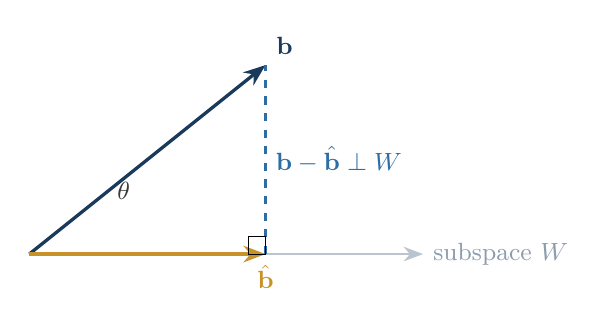
\begin{tikzpicture}
\draw[-{Stealth[length=7pt]},NavyBlue!30,thick] (0,0) -- (5,0) node[right,font=\small,color=NavyBlue!50]{subspace $W$};
\draw[-{Stealth[length=8pt]},NavyBlue,very thick] (0,0) -- (3,2.4) node[above right,font=\small]{$\mathbf{b}$};
\draw[-{Stealth[length=8pt]},Gold,very thick] (0,0) -- (3,0) node[below,font=\small]{$\hat{\mathbf{b}}$};
\draw[MidBlue,dashed,thick] (3,0) -- (3,2.4) node[midway,right,font=\small,color=MidBlue]{$\mathbf{b}-\hat{\mathbf{b}} \perp W$};
\draw (2.78,0) rectangle (3,0.22);
\node[font=\small,color=DarkGrey] at (1.2,0.8) {$\theta$};
\end{tikzpicture}
\end{center}

\subsection{Step 4: The Singular Value Decomposition}

\begin{problem}
Every $m\times n$ matrix $A$ can be written $A = U\Sigma V^T$ where $U$ is $m\times m$ orthogonal, $V$ is $n\times n$ orthogonal, and $\Sigma$ is $m\times n$ with non-negative entries $\sigma_1\geq\sigma_2\geq\cdots\geq 0$ on the main diagonal (the \textbf{singular values}).

\begin{enumerate}[label=(\alph*),topsep=2pt]
  \item \textbf{Deriving the SVD.} The matrix $A^TA$ is symmetric and positive semidefinite. Let $V$ be the orthogonal matrix that diagonalises it: $A^TA = V\Lambda V^T$. Define $\sigma_i = \sqrt{\lambda_i}$ and $\mathbf{u}_i = A\mathbf{v}_i/\sigma_i$. Show $\{\mathbf{u}_i\}$ are orthonormal and $AV = U\Sigma$.
  \item Compute the SVD of $A = \begin{pmatrix}3&2&2\\2&3&-2\end{pmatrix}$. Start by computing $A^TA$, finding its eigenvalues and eigenvectors.
  \item Write out $A = \sigma_1\mathbf{u}_1\mathbf{v}_1^T + \sigma_2\mathbf{u}_2\mathbf{v}_2^T + \cdots$ (outer product expansion). Each term is a rank-1 matrix. Verify for your example.
  \item Show that the columns of $V$ are eigenvectors of $A^TA$ and the columns of $U$ are eigenvectors of $AA^T$, with the same non-zero eigenvalues.
  \item The rank of $A$ equals the number of non-zero singular values. The condition number $\kappa(A) = \sigma_1/\sigma_r$ measures how sensitive the linear system $A\mathbf{x}=\mathbf{b}$ is to perturbations. What does a large condition number mean computationally?
\end{enumerate}
\end{problem}

\begin{thought}
\textbf{What the SVD sees.}
The SVD writes $A = U\Sigma V^T$, which says: every linear map from $\mathbb{R}^n$ to $\mathbb{R}^m$ is a rotation in the domain ($V^T$), followed by stretching along coordinate axes ($\Sigma$), followed by a rotation in the codomain ($U$). The singular values $\sigma_i$ are the stretching factors; the right singular vectors $\mathbf{v}_i$ are the input directions; the left singular vectors $\mathbf{u}_i$ are the output directions. If the spectral theorem says symmetric matrices have natural axes, the SVD says \emph{every} matrix has natural axes --- just in domain and codomain separately.
\end{thought}

\begin{problem}
\textbf{The best low-rank approximation.} The Eckart-Young theorem: the best rank-$k$ approximation to $A$ in terms of $\|A - B\|_F$ (Frobenius norm: $\|M\|_F^2 = \sum M_{ij}^2$) is $A_k = \sum_{i=1}^k\sigma_i\mathbf{u}_i\mathbf{v}_i^T$.

\begin{enumerate}[label=(\alph*),topsep=2pt]
  \item Show $\|A\|_F^2 = \sum\sigma_i^2 = \text{tr}(A^TA)$.
  \item The approximation error is $\|A - A_k\|_F^2 = \sum_{i>k}\sigma_i^2$. What fraction of the ``energy'' in $A$ is captured by the rank-$k$ approximation?
  \item For the matrix from Problem 4(b), compute $A_1$ (rank-1 approximation). How well does it approximate $A$?
  \item Apply to PCA: the top-$k$ SVD of the data matrix $X$ gives the same subspace as the top-$k$ eigenvectors of the covariance matrix. Show this connection explicitly.
  \item \textbf{Noise removal.} Suppose $A = A_{\text{signal}} + A_{\text{noise}}$ where the signal has low rank and the noise is small. Argue why truncating the SVD at rank $k$ separates signal from noise.
\end{enumerate}
\end{problem}

\begin{problem}
The pseudoinverse $A^+$ (from Module~2 deep problems) has a clean expression in terms of the SVD.
\begin{enumerate}[label=(\alph*),topsep=2pt]
  \item If $A = U\Sigma V^T$, define $A^+ = V\Sigma^+U^T$ where $\Sigma^+$ inverts the non-zero entries of $\Sigma$. Show $AA^+A = A$ and $A^+AA^+ = A^+$.
  \item For a full-rank $A$ with more rows than columns, show $A^+ = (A^TA)^{-1}A^T$ (the least-squares pseudoinverse from Module~2).
  \item A \textbf{regularised pseudoinverse} replaces $1/\sigma_i$ by $\sigma_i/(\sigma_i^2+\delta)$ for small $\delta>0$. Why does this stabilise the computation when some singular values are very small?
\end{enumerate}
\end{problem}

\begin{problem}
\textbf{Further applications.}
\begin{enumerate}[label=(\alph*),topsep=2pt]
  \item \textbf{Latent Semantic Analysis.} A document-term matrix $A$ has $A_{ij}=$ frequency of term $j$ in document $i$. The rank-$k$ SVD approximation groups documents and terms by ``topics.'' Describe what the left and right singular vectors represent in this context.
  \item \textbf{Numerical rank.} In practice, very small singular values can be due to noise. How would you decide whether a matrix of rank 5 with singular values $\{100, 80, 60, 40, 20, 0.001, 0.0003\}$ should be treated as rank 5 or rank 6?
  \item \textbf{Matrix norms.} The \textbf{spectral norm} (operator norm) of $A$ is $\|A\|_2 = \sigma_1$. The Frobenius norm is $\|A\|_F = \sqrt{\sum\sigma_i^2}$. Verify $\|A\|_2 \leq \|A\|_F \leq \sqrt{r}\|A\|_2$ where $r=\text{rank}(A)$.
\end{enumerate}
\end{problem}

\section{Part 3 \texorpdfstring{---}{--} Discovery}

\begin{discoverybox}
\textbf{What have we built?}

\textbf{First.} An inner product gives a vector space geometry: length, angle, and orthogonality. The Cauchy-Schwarz inequality bounds the angle between any two vectors.

\textbf{Second.} Gram-Schmidt turns any basis into an orthonormal one, producing the $QR$ decomposition. Orthonormal bases make projection trivial and computation stable.

\textbf{Third.} Orthogonal projection is the linear algebraic heart of least squares, PCA, and Fourier analysis: finding the best approximation of a vector by one lying in a subspace.

\textbf{Fourth.} The SVD $A = U\Sigma V^T$ decomposes every matrix as rotation--stretch--rotation. The singular values measure the ``size'' of the map in each independent direction. The Eckart-Young theorem makes truncated SVD the optimal low-rank approximation.

\medskip
\textbf{The thread to Journey 6.} The integral inner product $\langle f,g\rangle = \int fg$ makes $C[0,1]$ into an inner product space. The Fourier basis is orthonormal under this product. Expressing a function in this basis is the Fourier transform. Journey~6 will build that theory in full; but the linear algebraic foundation is already here.
\end{discoverybox}

\section{Part 4 \texorpdfstring{---}{--} Naming the Ideas}

\begin{namebox}
\textbf{Inner product space.}

An \textbf{inner product} satisfies symmetry, linearity in first slot, and positive-definiteness. It induces a norm $\|\mathbf{v}\|=\sqrt{\langle\mathbf{v},\mathbf{v}\rangle}$ and notion of angle.

\textbf{Cauchy-Schwarz}: $|\langle\mathbf{u},\mathbf{v}\rangle|\leq\|\mathbf{u}\|\|\mathbf{v}\|$.

\textbf{Orthonormal basis}: $\langle\mathbf{q}_i,\mathbf{q}_j\rangle=\delta_{ij}$. Expansion: $\mathbf{v}=\sum\langle\mathbf{v},\mathbf{q}_i\rangle\mathbf{q}_i$.

\textbf{Projection matrix}: $P=QQ^T$, satisfies $P^2=P$, $P^T=P$.
\end{namebox}

\begin{namebox}
\textbf{Singular Value Decomposition.}

$A = U\Sigma V^T$ with $U,V$ orthogonal and $\Sigma$ diagonal ($\sigma_1\geq\sigma_2\geq\cdots\geq 0$).

Columns of $V$: right singular vectors (eigenvectors of $A^TA$).\\
Columns of $U$: left singular vectors (eigenvectors of $AA^T$).\\
Diagonal entries of $\Sigma$: singular values $\sigma_i=\sqrt{\lambda_i(A^TA)}$.

\textbf{Best rank-$k$ approximation}: $A_k=\sum_{i=1}^k\sigma_i\mathbf{u}_i\mathbf{v}_i^T$ (Eckart-Young).

\textbf{Pseudoinverse}: $A^+=V\Sigma^+U^T$.
\end{namebox}

\section{Part 5 \texorpdfstring{---}{--} Deep Problems}

\begin{deepproblem}[Hilbert spaces and infinite dimensions]
A \textbf{Hilbert space} is an inner product space that is complete (every Cauchy sequence converges). $L^2[0,1]$ is the canonical example.
\begin{enumerate}[label=(\alph*)]
  \item The Fourier basis $\{e_n(x)=e^{2\pi inx}:n\in\mathbb{Z}\}$ is orthonormal in $L^2[0,1]$. Verify $\langle e_m,e_n\rangle=\delta_{mn}$.
  \item \textbf{Parseval's theorem}: for $f\in L^2[0,1]$ with Fourier coefficients $\hat{f}(n)=\langle f,e_n\rangle$, $\|f\|^2=\sum_{n=-\infty}^\infty|\hat{f}(n)|^2$. Interpret: the ``energy'' in $f$ equals the sum of squared Fourier coefficients.
  \item Use Parseval to evaluate $\sum_{n=1}^\infty 1/n^2$ by computing the Fourier series of $f(x)=x-1/2$ on $[0,1]$. (This is the Basel problem from Journey~1 Module~4, now solved by a completely different method.)
  \item An orthonormal set $\{e_n\}$ in a Hilbert space is a \textbf{complete basis} (Schauder basis) if every $f$ can be written $f=\sum\langle f,e_n\rangle e_n$ with convergence in norm. How does this differ from a finite-dimensional basis?
\end{enumerate}
\end{deepproblem}

\begin{deepproblem}[The SVD and the geometry of linear maps]
\begin{enumerate}[label=(\alph*)]
  \item Every $m\times n$ matrix $A$ with $m\geq n$ and rank $r$ maps the unit sphere $S^{n-1}$ to an ellipsoid in $\mathbb{R}^m$. Show the semi-axes of this ellipsoid are $\sigma_1\mathbf{u}_1,\ldots,\sigma_r\mathbf{u}_r$.
  \item The \textbf{Moore-Penrose conditions} characterise $A^+$ uniquely by four equations: $AA^+A=A$; $A^+AA^+=A^+$; $(AA^+)^T=AA^+$; $(A^+A)^T=A^+A$. Verify all four for $A^+=V\Sigma^+U^T$.
  \item Define the \textbf{nuclear norm} $\|A\|_* = \sum\sigma_i$ (sum of singular values). Show $\|A\|_* = \text{tr}(\sqrt{A^TA})$ (matrix square root). The nuclear norm is used in compressed sensing as a convex surrogate for rank. Why is minimising rank NP-hard while minimising $\|\cdot\|_*$ is tractable?
  \item A matrix $A$ satisfies $A^2=A$ if and only if $A$ is a projection matrix. Use the SVD to characterise all projection matrices: what must their singular values be?
\end{enumerate}
\end{deepproblem}

\begin{deepproblem}[Compressed sensing and sparse recovery]
A signal $\mathbf{x}\in\mathbb{R}^n$ is \textbf{$k$-sparse} if at most $k$ entries are non-zero. You observe $\mathbf{y}=A\mathbf{x}$ for a known $m\times n$ matrix $A$ with $m\ll n$ (far fewer measurements than unknowns).
\begin{enumerate}[label=(\alph*)]
  \item If $A$ is $m\times n$ with $m<n$, the system $A\mathbf{x}=\mathbf{y}$ is underdetermined: infinitely many solutions. Why cannot you recover $\mathbf{x}$ without additional information?
  \item The \textbf{compressed sensing recovery} problem: find the sparsest $\mathbf{x}$ satisfying $A\mathbf{x}=\mathbf{y}$, i.e.\ minimise $\|\mathbf{x}\|_0$ (number of non-zeros) subject to $A\mathbf{x}=\mathbf{y}$. This is NP-hard in general. The key insight: minimise $\|\mathbf{x}\|_1=\sum|x_i|$ instead. Under the \textbf{restricted isometry property} (RIP), $\ell^1$ minimisation recovers the true sparse solution exactly. Explain geometrically why $\ell^1$ promotes sparsity while $\ell^2$ does not. (Compare unit balls in $\mathbb{R}^2$.)
  \item The RIP requires $A$ to act nearly isometrically on all $k$-sparse vectors: $(1-\delta)\|\mathbf{x}\|^2\leq\|A\mathbf{x}\|^2\leq(1+\delta)\|\mathbf{x}\|^2$. Gaussian random matrices satisfy RIP with high probability when $m=O(k\log(n/k))$. Why is randomness useful here?
  \item Name one application of compressed sensing in medical imaging or communications. What constraint does it relax?
\end{enumerate}
\end{deepproblem}

\section{Part 6 \texorpdfstring{---}{--} Reflection}

\begin{reflectionbox}
\textbf{Your reflection task.}

\begin{enumerate}
  \item \textbf{On geometry and algebra.} The inner product imports geometry (length, angle) into the abstract algebraic world of vector spaces. But ``length'' and ``angle'' are physical concepts. Write a paragraph: does the inner product reveal that algebra and geometry were always the same, or does it impose a geometric interpretation onto an algebraic structure?

  \item \textbf{On the SVD.} The SVD says every linear map is a composition of two rotations and a scaling. Rotations preserve shape; only the scaling distorts. What does this say about the nature of linear transformations --- are they fundamentally simpler than they look?

  \item \textbf{On compression.} Image compression via SVD keeps only the top $k$ singular values. What is discarded? Is there a sense in which the discarded information is ``unimportant''? Who decides what counts as unimportant, and what could go wrong in applications where this decision is made automatically?

  \item \textbf{Looking ahead.} Module 5 studies linear maps on inner product spaces more deeply --- in particular, the adjoint of an operator and the spectral theorem in full generality. You have seen that symmetric matrices have real eigenvalues and orthogonal eigenvectors. What is the right generalisation of ``symmetric'' for an arbitrary linear map on an inner product space?
\end{enumerate}
\end{reflectionbox}

\medskip
\noindent\textbf{Looking ahead.}
Module~5 completes the linear algebra of inner product spaces: the adjoint, normal operators, and the full spectral theorem. Module~6 closes Journey~3 by connecting everything to systems of differential equations and the structure of solution spaces.

\vspace{1.4cm}
\begin{center}
{\color{MidBlue}\rule{0.5\linewidth}{0.8pt}}\\[6pt]
{\small\color{DarkGrey}\textit{End of Journey 3, Module 4 --- Inner Products and the SVD}}\\[4pt]
{\small\color{DarkGrey}Continue to: \textbf{Module 5 --- Adjoints and the Spectral Theorem}}\\[6pt]
{\color{MidBlue}\rule{0.5\linewidth}{0.8pt}}
\end{center}

\end{document}